\chapter{Rigid Multibody Dynamics}
\label{chp:back_RBDynamics}

In this chapter, a mathematical groundwork for characterizing the dynamics of a floating-base multibody system is presented, setting a convention that is used throughout this work. Then, a first introduction to recursive algorithms for the computation of the dynamics of a multibody system is presented, to give a comprehensive understanding of the state of the art in the field of rigid multibody dynamics algorithms. In the forthcoming discussion, a 6D \textit{spatial vectors} notation firstly introduced by \citet{featherstone_rigid_2008} and successively integrated and adapted by \citet{traversaro_multibody_2019} is presented. As a matter of fact, this notation allows us to describe the motion of a rigid body without excessive use of indices, which can be confusing and error-prone when dealing with complex recursive algorithms that will be further discussed. This convention will be used to describe the kinematics and dynamics of a floating-base multibody system in a unified manner throughout this work.

\section{Formalisms and Notation}

\paragraph{Spatial Vectors} A spatial vector is a 6D vector that describes the motion of a rigid body in space.

\begin{figure}
    \centering
    \caption{Velocity of rigid body expressed in terms of spatial vectors.}
    \tikzset{every picture/.style={line width=0.75pt}}
    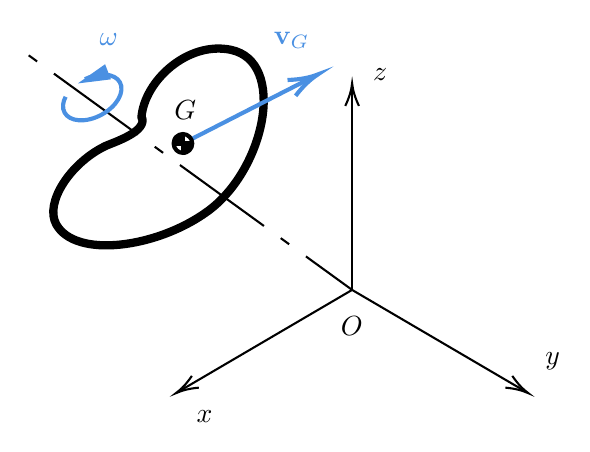
\begin{tikzpicture}[x=0.75pt,y=0.75pt,yscale=-1,xscale=1]
        \draw [color={rgb, 255:red, 0; green, 0; blue, 0 }  ,draw opacity=1 ]   (379.99,208.64) -- (379.99,111.06) ;
        \draw [shift={(379.99,109.06)}, rotate = 90] [color={rgb, 255:red, 0; green, 0; blue, 0 }  ,draw opacity=1 ][line width=0.75]    (10.93,-3.29) .. controls (6.95,-1.4) and (3.31,-0.3) .. (0,0) .. controls (3.31,0.3) and (6.95,1.4) .. (10.93,3.29)   ;
        \draw [color={rgb, 255:red, 0; green, 0; blue, 0 }  ,draw opacity=1 ]   (379.98,208.64) -- (463.22,257.42) ;
        \draw [shift={(464.94,258.43)}, rotate = 210.37] [color={rgb, 255:red, 0; green, 0; blue, 0 }  ,draw opacity=1 ][line width=0.75]    (10.93,-3.29) .. controls (6.95,-1.4) and (3.31,-0.3) .. (0,0) .. controls (3.31,0.3) and (6.95,1.4) .. (10.93,3.29)   ;
        \draw [color={rgb, 255:red, 0; green, 0; blue, 0 }  ,draw opacity=1 ]   (379.99,208.64) -- (338.26,233.09) -- (296.75,257.42) ;
        \draw [shift={(295.03,258.43)}, rotate = 329.63] [color={rgb, 255:red, 0; green, 0; blue, 0 }  ,draw opacity=1 ][line width=0.75]    (10.93,-3.29) .. controls (6.95,-1.4) and (3.31,-0.3) .. (0,0) .. controls (3.31,0.3) and (6.95,1.4) .. (10.93,3.29)   ;
        \draw  [line width=3] [line join = round][line cap = round] (278.46,125.78) .. controls (279.81,107.79) and (300.93,88.72) .. (321.49,92.95) .. controls (348.63,98.54) and (338.39,150.24) .. (310.57,170.62) .. controls (286.05,188.57) and (246.65,193.72) .. (237.42,177.02) .. controls (231.68,166.64) and (244.3,147.49) .. (261,139.39) .. controls (264.29,137.79) and (282.45,132.22) .. (278.45,124.98) ;
        \draw [color={rgb, 255:red, 0; green, 0; blue, 0 }  ,draw opacity=1 ] [dash pattern={on 3.75pt off 7.5pt on 37.5pt off 7.5pt}]  (224.18,95.63) -- (379.99,208.64) ;
        \draw  [draw opacity=0][line width=1.5]  (247.83,109.17) .. controls (250.15,107.51) and (252.87,106.21) .. (255.73,105.49) .. controls (263.49,103.53) and (269.36,106.62) .. (268.84,112.38) .. controls (268.32,118.15) and (261.61,124.41) .. (253.85,126.36) .. controls (246.09,128.32) and (240.22,125.23) .. (240.74,119.46) .. controls (240.85,118.18) and (241.28,116.87) .. (241.95,115.59) -- (254.79,115.92) -- cycle ; \draw [color={rgb, 255:red, 74; green, 144; blue, 226 }  ,draw opacity=1 ][line width=1.5]    (251.3,107.11) .. controls (252.71,106.43) and (254.2,105.87) .. (255.73,105.49) .. controls (263.49,103.53) and (269.36,106.62) .. (268.84,112.38) .. controls (268.32,118.15) and (261.61,124.41) .. (253.85,126.36) .. controls (246.09,128.32) and (240.22,125.23) .. (240.74,119.46) .. controls (240.85,118.18) and (241.28,116.87) .. (241.95,115.59) ;  \draw [shift={(247.83,109.17)}, rotate = 338.9] [fill={rgb, 255:red, 74; green, 144; blue, 226 }  ,fill opacity=1 ][line width=0.08]  [draw opacity=0] (15.6,-3.9) -- (0,0) -- (15.6,3.9) -- cycle    ;
        \draw [color={rgb, 255:red, 74; green, 144; blue, 226 }  ,draw opacity=1 ][line width=1.5]    (298.49,138.09) -- (360.8,106.21) ;
        \draw [shift={(363.47,104.84)}, rotate = 152.9] [color={rgb, 255:red, 74; green, 144; blue, 226 }  ,draw opacity=1 ][line width=1.5]    (14.21,-4.28) .. controls (9.04,-1.82) and (4.3,-0.39) .. (0,0) .. controls (4.3,0.39) and (9.04,1.82) .. (14.21,4.28)   ;
        \draw  [fill={rgb, 255:red, 255; green, 255; blue, 255 }  ,fill opacity=1 ][line width=1.5]  (294,138.09) .. controls (294,135.58) and (296.01,133.55) .. (298.49,133.55) .. controls (300.97,133.55) and (302.98,135.58) .. (302.98,138.09) .. controls (302.98,140.61) and (300.97,142.64) .. (298.49,142.64) .. controls (296.01,142.64) and (294,140.61) .. (294,138.09) -- cycle ; \draw  [line width=1.5]  (294,138.09) -- (302.98,138.09) ; \draw  [line width=1.5]  (298.49,133.55) -- (298.49,142.64) ;
        \draw  [line width=1.5] [line join = round][line cap = round] (299.1,138.58) .. controls (299.08,138.83) and (298.95,139.56) .. (298.95,139.31) .. controls (298.95,139.18) and (300.23,138.76) .. (300.33,138.37) .. controls (300.4,138.11) and (299.1,139.02) .. (299.26,139) .. controls (301.37,138.71) and (299.1,138.8) .. (298.95,139.88) .. controls (298.93,140.04) and (299.87,139.36) .. (299.98,139.31) .. controls (300.53,139.05) and (301.15,138.88) .. (301.62,138.48) .. controls (301.72,138.38) and (301.34,138.54) .. (301.21,138.58) .. controls (301,138.64) and (299.91,138.85) .. (300.08,139.1) .. controls (300.21,139.31) and (301.92,137.93) .. (301.82,138.79) .. controls (301.78,139.21) and (301.08,139.16) .. (300.69,139.31) .. controls (300.63,139.33) and (300.78,139.19) .. (300.85,139.15) .. controls (301.22,138.95) and (301.84,138.49) .. (302.08,138.84) .. controls (302.32,139.2) and (301.99,140.26) .. (301.41,139.67) .. controls (301.21,139.47) and (301.48,138.55) .. (301.87,138.89) .. controls (302.89,139.77) and (301.81,139.71) .. (301.67,139.52) .. controls (301.17,138.85) and (302.72,138.36) .. (302.75,138.53) .. controls (302.81,138.9) and (302.06,138.96) .. (301.93,139.31) .. controls (301.82,139.58) and (301.96,139.91) .. (301.87,140.19) .. controls (301.77,140.55) and (301.51,140.84) .. (301.36,141.18) .. controls (301.31,141.3) and (301.24,141.67) .. (301.26,141.54) .. controls (301.47,140.39) and (301.63,139) .. (302.28,138.01) .. controls (302.6,137.53) and (301.78,139.04) .. (301.46,139.52) .. controls (301.23,139.87) and (300.44,140.84) .. (300.75,140.56) .. controls (303.14,138.35) and (301.15,140.3) .. (300.54,140.92) .. controls (300.32,141.14) and (300.81,140.36) .. (300.95,140.09) .. controls (301.06,139.87) and (301.25,139.69) .. (301.36,139.47) .. controls (301.44,139.3) and (301.16,139.78) .. (301.05,139.93) .. controls (300.7,140.42) and (300.28,140.86) .. (299.92,141.34) .. controls (299.88,141.4) and (299.45,142.32) .. (299.15,142.17) .. controls (299.05,142.12) and (299.67,140.21) .. (300.18,140.04) .. controls (300.33,139.99) and (300.06,140.33) .. (299.98,140.45) .. controls (299.51,141.13) and (298.91,141.7) .. (298.44,142.38) .. controls (298.4,142.42) and (298.57,142.38) .. (298.59,142.32) .. controls (298.8,141.66) and (298.96,140.98) .. (299.1,140.3) .. controls (299.14,140.11) and (299.09,139.54) .. (299.15,139.73) .. controls (299.24,139.97) and (299.12,140.76) .. (299.1,140.51) .. controls (299.08,140.2) and (299.07,139.52) .. (299.36,139.62) .. controls (299.89,139.8) and (299.57,141.04) .. (299.57,141.13) .. controls (299.56,141.27) and (299.42,140.85) .. (299.46,140.71) .. controls (299.59,140.27) and (299.79,139.85) .. (299.92,139.41) .. controls (299.94,139.35) and (299.84,139.51) .. (299.82,139.57) .. controls (299.75,139.84) and (299.77,140.14) .. (299.67,140.4) .. controls (299.51,140.82) and (299.4,141.31) .. (299.05,141.6) .. controls (298.87,141.75) and (299.02,141.1) .. (299.1,140.87) .. controls (299.17,140.7) and (300.17,139.73) .. (300.08,139.78) .. controls (299.59,140.02) and (299.41,140.9) .. (299.41,141.44) .. controls (299.41,141.48) and (299.42,141.54) .. (299.46,141.54) .. controls (299.51,141.54) and (299.54,141.49) .. (299.57,141.44) .. controls (299.91,140.69) and (300.2,140.03) .. (300.69,139.36) .. controls (300.75,139.29) and (300.57,139.49) .. (300.54,139.57) .. controls (300.27,140.22) and (300.09,141) .. (299.67,141.6) .. controls (299.63,141.65) and (299.64,141.45) .. (299.67,141.39) .. controls (299.83,141.06) and (300.01,140.74) .. (300.23,140.45) .. controls (300.44,140.18) and (300.74,140) .. (300.95,139.73) .. controls (301,139.66) and (300.94,139.39) .. (300.9,139.47) .. controls (300.56,140.1) and (300.25,140.76) .. (299.82,141.34) .. controls (299.6,141.63) and (298.9,142.47) .. (299.1,142.17) .. controls (299.86,141.02) and (300.02,141.19) .. (301.1,140.3) .. controls (301.16,140.25) and (300.94,140.34) .. (300.9,140.4) .. controls (300.8,140.55) and (300.74,140.72) .. (300.64,140.87) .. controls (300.2,141.53) and (299.56,142.02) .. (299,142.58) .. controls (298.3,143.3) and (300.67,141.48) .. (301.41,140.82) .. controls (301.57,140.67) and (301.89,140.11) .. (301.72,140.25) .. controls (300.81,140.94) and (300.05,141.82) .. (299.15,142.53) .. controls (299.08,142.59) and (299.34,142.45) .. (299.41,142.38) .. controls (299.73,142.06) and (300,141.69) .. (300.33,141.39) .. controls (300.7,141.07) and (302.03,140.52) .. (302.03,139.73) .. controls (302.03,139.61) and (301.87,139.72) .. (301.87,139.73) .. controls (301.52,140.19) and (300.15,142.04) .. (299.98,141.6) .. controls (299.76,141.05) and (299.98,140.42) .. (300.03,139.83) .. controls (300.04,139.6) and (299.87,139.31) .. (300.03,139.15) ;
        \draw  [line width=1.5] [line join = round][line cap = round] (300.23,139.57) .. controls (300.19,139.35) and (300.18,139.1) .. (300.03,138.95) ;
        \draw  [line width=1.5] [line join = round][line cap = round] (294.23,137.49) .. controls (295.32,137.47) and (296.42,137.48) .. (297.51,137.44) .. controls (297.75,137.43) and (298.19,137.58) .. (298.23,137.33) .. controls (298.43,136.28) and (298.22,135.18) .. (298.13,134.11) .. controls (298.07,133.49) and (297.36,134.34) .. (297.31,134.37) .. controls (295.99,135.17) and (295.72,135.35) .. (295.1,136.55) .. controls (294.96,136.82) and (294.37,137.2) .. (294.64,137.33) .. controls (295.32,137.68) and (295.39,137.16) .. (296.02,137.07) .. controls (296.58,137) and (297.15,137.11) .. (297.72,137.07) .. controls (298.08,137.05) and (297.64,136.35) .. (297.67,135.98) .. controls (297.7,135.39) and (298.11,134.76) .. (297.87,134.22) .. controls (297.73,133.9) and (297.53,134.84) .. (297.26,135.05) .. controls (296.81,135.39) and (296.14,135.41) .. (295.77,135.83) .. controls (295.43,136.21) and (295.43,136.8) .. (295.25,137.28) .. controls (295.23,137.35) and (295.26,137.13) .. (295.31,137.07) .. controls (295.51,136.8) and (295.78,136.58) .. (295.97,136.29) .. controls (296.33,135.76) and (296.78,135.28) .. (297.26,134.84) .. controls (297.31,134.79) and (297.11,134.81) .. (297.05,134.84) .. controls (296.69,135.02) and (296.29,135.16) .. (296.02,135.46) .. controls (295.57,135.98) and (294.41,136.8) .. (294.95,137.23) .. controls (295.63,137.79) and (297.74,134.95) .. (297.97,134.68) .. controls (298.03,134.63) and (297.93,134.84) .. (297.87,134.89) .. controls (297.58,135.16) and (296.02,135.89) .. (296.02,136.81) .. controls (296.02,137.4) and (296.8,135.93) .. (297.26,135.57) .. controls (297.38,135.47) and (297.25,135.91) .. (297.15,136.03) .. controls (296.9,136.39) and (295.97,136.71) .. (296.28,137.02) .. controls (296.6,137.34) and (297.06,136.58) .. (297.41,136.29) .. controls (297.46,136.25) and (297.25,136.29) .. (297.2,136.35) .. controls (296.95,136.69) and (296.77,137.08) .. (296.54,137.44) .. controls (296.53,137.45) and (296.47,137.44) .. (296.49,137.44) .. controls (297.11,137.44) and (298.38,135.81) .. (297.97,136.29) .. controls (297.65,136.68) and (296.65,137.08) .. (297,137.44) .. controls (297.32,137.77) and (297.63,136.76) .. (297.97,136.45) .. controls (298.04,136.39) and (298,136.63) .. (297.97,136.71) .. controls (297.93,136.91) and (297.77,137.08) .. (297.77,137.28) .. controls (297.77,137.38) and (297.88,137.07) .. (297.97,137.07) .. controls (298.22,137.07) and (298.36,137.62) .. (298.18,137.8) ;
        \draw  [line width=1.5] [line join = round][line cap = round] (298.08,135.72) .. controls (297.92,135.83) and (297.77,135.93) .. (297.62,136.03) ;
        \draw  [line width=1.5] [line join = round][line cap = round] (294.84,135.31) .. controls (295.22,135.37) and (295.1,136.07) .. (295.05,136.45) .. controls (295.04,136.48) and (295.03,136.58) .. (295.05,136.55) .. controls (295.33,136.27) and (295.24,136.14) .. (295.41,135.77) .. controls (295.48,135.63) and (295.59,135.51) .. (295.67,135.36) .. controls (295.71,135.27) and (295.9,135.04) .. (295.82,135.1) .. controls (295.46,135.39) and (295.18,135.68) .. (294.79,135.93) ;
        \draw (303.64,265.06) node [anchor=north west][inner sep=0.75pt]  [color={rgb, 255:red, 0; green, 0; blue, 0 }  ,opacity=1 ]  {$x$};
        \draw (471.61,237.21) node [anchor=north west][inner sep=0.75pt]  [color={rgb, 255:red, 0; green, 0; blue, 0 }  ,opacity=1 ]  {$y$};
        \draw (388.63,100.33) node [anchor=north west][inner sep=0.75pt]  [color={rgb, 255:red, 0; green, 0; blue, 0 }  ,opacity=1 ]  {$z$};
        \draw (373.1,219.89) node [anchor=north west][inner sep=0.75pt]    {$O$};
        \draw (256.8,83.8) node [anchor=north west][inner sep=0.75pt]  [color={rgb, 255:red, 74; green, 144; blue, 226 }  ,opacity=1 ]  {$\omega $};
        \draw (340.8,82.8) node [anchor=north west][inner sep=0.75pt]  [color={rgb, 255:red, 74; green, 144; blue, 226 }  ,opacity=1 ]  {$\mathbf{v}_{G}$};
        \draw (292.8,115.8) node [anchor=north west][inner sep=0.75pt]    {$G$};
    \end{tikzpicture}
\end{figure}

In the case of a rigid body, the velocity of a point $G$ attached to the body with respect to an intertial reference frame attached to an arbitrary point $O$ in the space can be generally expressed by its angular component $\omega$ about an axis passing through $O$ and its linear component $v _A$, for which the following relation holds:

\begin{equation}
    v _A = \omega \times {}^O R_G
\end{equation}

where ${}^O R_G$ is the position vector of $G$ with respect to $O$. This holds for any point $G$ on the rigid body. In order to simplify the notation, introducing a Cartesian coordinate frame $\mathcal{O} _{xyz}$, we can define a basis of 6 spatial vectors $\mathcal{D} _O = \{\mathbf{d} _i\} ^6 _{i=1}$ as:

\begin{equation}
    \mathcal{D} _O = \{\mathbf{d} _x, \mathbf{d} _y, \mathbf{d} _z, \mathbf{d} _{O _x}, \mathbf{d} _{O _y}, \mathbf{d} _{O _z} \} \subset \mathcal{M} ^6
\end{equation}

where $\mathcal{M} ^6$ is the space of 6D vectors, defining a Pl\"ucker coordinate system on $\mathcal{M} ^6$ as shown in \cref{fig:pluecker}.

% === Fig: Pluecker === %
\begin{figure}
    \centering
    \caption{Pl\"ucker motion coordinate system}
    \label{fig:pluecker}
    \tikzset{every picture/.style={line width=0.75pt}}
    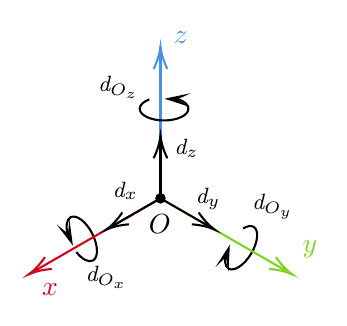
\begin{tikzpicture}[x=0.75pt,y=0.75pt,yscale=-1,xscale=1]
        \draw [color={rgb, 255:red, 74; green, 144; blue, 226 }  ,draw opacity=1 ]   (249.79,80.38) -- (249.79,9.08) ;
        \draw [shift={(249.79,7.08)}, rotate = 90] [color={rgb, 255:red, 74; green, 144; blue, 226 }  ,draw opacity=1 ][line width=0.75]    (10.93,-3.29) .. controls (6.95,-1.4) and (3.31,-0.3) .. (0,0) .. controls (3.31,0.3) and (6.95,1.4) .. (10.93,3.29)   ;
        \draw  [draw opacity=0] (257.99,32.5) .. controls (261.16,33.51) and (263.25,35.24) .. (263.25,37.21) .. controls (263.25,40.32) and (258,42.85) .. (251.52,42.85) .. controls (245.05,42.85) and (239.8,40.32) .. (239.8,37.21) .. controls (239.8,35.38) and (241.61,33.75) .. (244.41,32.72) -- (251.52,37.21) -- cycle ; \draw   (257.99,32.5) .. controls (261.16,33.51) and (263.25,35.24) .. (263.25,37.21) .. controls (263.25,40.32) and (258,42.85) .. (251.52,42.85) .. controls (245.05,42.85) and (239.8,40.32) .. (239.8,37.21) .. controls (239.8,35.38) and (241.61,33.75) .. (244.41,32.72) ;
        \draw  [draw opacity=0] (205.05,97.73) .. controls (204.06,93.79) and (204.55,90.48) .. (206.55,89.46) .. controls (209.33,88.05) and (213.96,91.58) .. (216.9,97.35) .. controls (219.84,103.12) and (219.97,108.94) .. (217.19,110.35) .. controls (215.09,111.42) and (211.93,109.66) .. (209.25,106.25) -- (211.87,99.91) -- cycle ; \draw   (205.05,97.73) .. controls (204.06,93.79) and (204.55,90.48) .. (206.55,89.46) .. controls (209.33,88.05) and (213.96,91.58) .. (216.9,97.35) .. controls (219.84,103.12) and (219.97,108.94) .. (217.19,110.35) .. controls (215.09,111.42) and (211.93,109.66) .. (209.25,106.25) ;
        \draw  [draw opacity=0] (289.6,94.92) .. controls (291.53,93.69) and (293.37,93.33) .. (294.68,94.12) .. controls (297.34,95.72) and (296.8,101.52) .. (293.45,107.07) .. controls (290.11,112.61) and (285.24,115.81) .. (282.57,114.2) .. controls (280.67,113.05) and (280.4,109.78) .. (281.61,105.98) -- (288.62,104.16) -- cycle ; \draw   (289.6,94.92) .. controls (291.53,93.69) and (293.37,93.33) .. (294.68,94.12) .. controls (297.34,95.72) and (296.8,101.52) .. (293.45,107.07) .. controls (290.11,112.61) and (285.24,115.81) .. (282.57,114.2) .. controls (280.67,113.05) and (280.4,109.78) .. (281.61,105.98) ;
        \draw  [fill={rgb, 255:red, 0; green, 0; blue, 0 }  ,fill opacity=1 ] (205.98,94.78) -- (206.86,101.37) -- (202.81,96.09) -- (205.63,98.4) -- cycle ;
        \draw  [fill={rgb, 255:red, 0; green, 0; blue, 0 }  ,fill opacity=1 ] (279.01,110.18) -- (282.61,104.59) -- (282.28,111.23) -- (281.63,107.65) -- cycle ;
        \draw  [fill={rgb, 255:red, 0; green, 0; blue, 0 }  ,fill opacity=1 ] (260,34.53) -- (253.67,32.48) -- (260.18,31.11) -- (256.88,32.65) -- cycle ;
        \draw [color={rgb, 255:red, 126; green, 211; blue, 33 }  ,draw opacity=1 ]   (249.79,80.38) -- (311.53,116.02) ;
        \draw [shift={(313.27,117.02)}, rotate = 210] [color={rgb, 255:red, 126; green, 211; blue, 33 }  ,draw opacity=1 ][line width=0.75]    (10.93,-3.29) .. controls (6.95,-1.4) and (3.31,-0.3) .. (0,0) .. controls (3.31,0.3) and (6.95,1.4) .. (10.93,3.29)   ;
        \draw [color={rgb, 255:red, 208; green, 2; blue, 27 }  ,draw opacity=1 ]   (249.79,80.37) -- (218.61,98.38) -- (188.04,116.02) ;
        \draw [shift={(186.31,117.02)}, rotate = 330] [color={rgb, 255:red, 208; green, 2; blue, 27 }  ,draw opacity=1 ][line width=0.75]    (10.93,-3.29) .. controls (6.95,-1.4) and (3.31,-0.3) .. (0,0) .. controls (3.31,0.3) and (6.95,1.4) .. (10.93,3.29)   ;
        \draw    (249.79,80.38) -- (249.79,52.13) ;
        \draw [shift={(249.79,50.13)}, rotate = 90] [color={rgb, 255:red, 0; green, 0; blue, 0 }  ][line width=0.75]    (10.93,-3.29) .. controls (6.95,-1.4) and (3.31,-0.3) .. (0,0) .. controls (3.31,0.3) and (6.95,1.4) .. (10.93,3.29)   ;
        \draw    (249.79,80.38) -- (274.25,94.5) ;
        \draw [shift={(275.99,95.5)}, rotate = 210] [color={rgb, 255:red, 0; green, 0; blue, 0 }  ][line width=0.75]    (10.93,-3.29) .. controls (6.95,-1.4) and (3.31,-0.3) .. (0,0) .. controls (3.31,0.3) and (6.95,1.4) .. (10.93,3.29)   ;
        \draw    (249.79,80.37) -- (225.32,94.5) ;
        \draw [shift={(223.59,95.5)}, rotate = 330] [color={rgb, 255:red, 0; green, 0; blue, 0 }  ][line width=0.75]    (10.93,-3.29) .. controls (6.95,-1.4) and (3.31,-0.3) .. (0,0) .. controls (3.31,0.3) and (6.95,1.4) .. (10.93,3.29)   ;
        \draw (191.23,119.9) node [anchor=north west][inner sep=0.75pt]  [color={rgb, 255:red, 208; green, 2; blue, 27 }  ,opacity=1 ]  {$x$};
        \draw (316.73,99.4) node [anchor=north west][inner sep=0.75pt]  [color={rgb, 255:red, 126; green, 211; blue, 33 }  ,opacity=1 ]  {$y$};
        \draw (254.73,-1.35) node [anchor=north west][inner sep=0.75pt]  [color={rgb, 255:red, 74; green, 144; blue, 226 }  ,opacity=1 ]  {$z$};
        \draw (212.25,111.65) node [anchor=north west][inner sep=0.75pt]  [font=\footnotesize]  {$\mathit{d}_{O_{x}}$};
        \draw (218.25,20.15) node [anchor=north west][inner sep=0.75pt]  [font=\footnotesize]  {$\mathit{d}_{O_{z}}$};
        \draw (292.5,76.9) node [anchor=north west][inner sep=0.75pt]  [font=\footnotesize]  {$\mathit{d}_{O_{y}}$};
        \draw (255,50.4) node [anchor=north west][inner sep=0.75pt]  [font=\footnotesize]  {$\mathit{d}_{z}$};
        \draw (225.25,70.9) node [anchor=north west][inner sep=0.75pt]  [font=\footnotesize]  {$\mathit{d}_{x}$};
        \draw (265.25,73.9) node [anchor=north west][inner sep=0.75pt]  [font=\footnotesize]  {$\mathit{d}_{y}$};
        \draw (242.75,86.65) node [anchor=north west][inner sep=0.75pt]    {$O$};
        \draw [fill={rgb, 255:red, 0; green, 0; blue, 0 }  ,fill opacity=1 ]  (249.79, 80.38) circle [x radius= 2, y radius= 2]   ;
    \end{tikzpicture}
\end{figure}

\paragraph{Spatial Subspace} Once defined $\mathcal{M} ^n$ as a vector space, we can define a subset $\boldsymbol{\Phi} \subset \mathcal{M} ^n$, which is also a vector space. Given a constraint matrix $\mathbf{K} \in \mathbb{R} ^{m \times n}$ with $m$ number of constraints and $n$ number of degrees of freedom, then we can define the subspace $\boldsymbol{\Phi}$ as the null space of $\mathbf{K}$:

\begin{equation}
    \boldsymbol{\Phi} = \ker (\mathbf{K})
\end{equation}

This defines a motion subspace for a system, e.g. defines the directions in which the system is free to move.

\paragraph{Spatial Velocity} The spatial velocity of a rigid body is defined as a serialization of the linear and angular velocity of a point $A$ attached to the body. In particular, let $\mathbf{p} _A \in \mathcal{D}_O$ be the pose vector of $A$ with respect to $O$, then the spatial velocity of the body is defined as the component-wise derivative of the spatial vector respect to time:

\begin{equation}
    \mathbf{v} _A = \frac{d}{dt} {}^{[O]}\mathbf{p} _A =
    \lim _{\delta t \to 0} \frac{1}{\delta t}
    \begin{bmatrix}
        p _{A _x} (t + \delta t)     & - & p _{A _x} (t)     \\
        p _{A _y} (t + \delta t)     & - & p _{A _y} (t)     \\
        p _{A _z} (t + \delta t)     & - & p _{A _z} (t)     \\
        p _{A _{O_x}} (t + \delta t) & - & p _{A _{O_x}} (t) \\
        p _{A _{O_y}} (t + \delta t) & - & p _{A _{O_y}} (t) \\
        p _{A _{O_z}} (t + \delta t) & - & p _{A _{O_z}} (t) \\
    \end{bmatrix}
    = \begin{bmatrix}
        v _A \\
        \omega _A
    \end{bmatrix}
\end{equation}

\paragraph{Spatial Acceleration} Given that the spatial velocity decouples the linear and angular components of the motion, defining a property of the body as a whole and not of a single body-fixed point, the spatial acceleration of a rigid body is defined as simply as just the time derivative of its spatial velocity:

\begin{equation}
    \dot{\mathbf{v}} _A = \frac{d}{dt} \begin{bmatrix}
        v _A (t) \\
        \omega (t)
    \end{bmatrix}
    =
    \begin{bmatrix}
        \dot{v} _A \\
        \dot{\omega}
    \end{bmatrix}
\end{equation}

\paragraph{Spatial Forces} The spatial force acting on a rigid body is defined, in a similar manner as the spatial velocity as a stacking of the linear component $f \in \mathbb{R}^3$ and the angular component $\tau \in \mathbb{R}^3$ of the wrench acting on the body, in particular, we can defined $\mathbf{f} \in \mathbb{R}^6$ respect to a frame $B$ in relation to its motion as:

\begin{equation}
    {}_{B}\mathbf{f} = \begin{bmatrix}
        {}_{B}f \\
        {}_{B}\tau
    \end{bmatrix}
\end{equation}

\paragraph{Multibody Velocity} Given a floating-base multibody system composed of $n$ rigid bodies, we can define the velocity of the system as the concatenation of the root link velocity $\mathbf{v}_A$ and the velocities of each body composing the system $\dot{\mathbf{s}} \in \mathbb{R} ^{n}$:

\begin{equation}
    \boldsymbol{\nu} = \begin{bmatrix}
        \begin{bmatrix} v _a \\ \omega _A \end{bmatrix} \\
        \dot{\mathbf{s}}                                \\
    \end{bmatrix} = \begin{bmatrix}
        \mathbf{v}_A \\
        \dot{\mathbf{s}}
    \end{bmatrix}
\end{equation}

\paragraph{Multibody Acceleration} Similarly, the acceleration of the floating-base system can be defined as the concatenation of the acceleration of the root link $\dot{\mathbf{v}} _A$ and the accelerations of each body composing the system $\ddot{\mathbf{s}} \in \mathbb{R} ^{n}$:

\begin{equation}
    \dot{\boldsymbol{\nu _A}} = \begin{bmatrix}
        \begin{bmatrix} \dot{v} _a \\ \dot{\omega} _A \end{bmatrix} \\
        \ddot{\mathbf{s}}                                           \\
    \end{bmatrix} = \begin{bmatrix}
        \dot{\mathbf{v}}_A \\
        \ddot{\mathbf{s}}
    \end{bmatrix}
\end{equation}

\section{Multibody Kinematics}

\subsection{Joints and Links}

A multibody kinematic tree can be described as a contiguous assembly of two main physical elements: links and joints. The links correspond to the rigid bodies composing the inertial properties of the system, while the joints are usually modeled as massless elements connecting two links, allowing relative motion between them. They are classified according to the number of \ac{DoF} they allow, which is the number of independent coordinates needed to describe the relative motion between the two links, usually assuming values between 0 (fixed joint) and 6 (free joint).

For the sake of simplicity and without loss of generality, in this work, only 1-\ac{DoF} joint will be considered, as their properties can be easily extended to multidimensional cases. Furthermore, the system will be considered \textit{acyclic}, i.e. it will not contain any closed loop, as the presence of loops would make the system kinematically redundant.
Given a joint we can define a \textit{joint axis} $\mathbf{a} \in \mathbb{R}^3, |\mathbf{a}| = 1$ with $\mathbf{a}^\wedge \mathbf{a} = \mathbbm{0}_{3 \times 1}$, in this case, if we recall the definition of the spatial subspace, we can define the joint motion subspace $\boldsymbol{\Phi} _j \in \mathcal{M} ^6$ as:

\begin{equation}
    \boldsymbol{\Phi} _j =
    \begin{cases}
        [\mathbbm{0}_{1 \times 6}] ^\top             & \text{if the joint is fixed}     \\
        [\mathbf{a}, \mathbbm{0}_{1 \times 3}] ^\top & \text{if the joint is prismatic} \\
        [\mathbbm{0}_{1 \times 3}, \mathbf{a}] ^\top & \text{if the joint is revolute}
    \end{cases}
\end{equation}

\section{Equation of Motion}
\label{sec:back_eom}

When dealing with a multi-body system, the configuration must be described in non-Euclidean space by a configuration belonging to a smooth manifold ${}^W\mathbf{H} \in \mathbb{Q}:\mathrm{SE}(3)\times\mathbb{R}^n$ where $H$ is the pose of the system and $n$ is the number of \ac{DoF} of the system and $\mathrm{SE}(3)$ is the \textit{special Euclidean} Lie group defined as:

\begin{equation}
    \mathrm{SE}(3) := \left\{
    \begin{bmatrix}
        R                         & p \\
        \mathbbm{0} _{1 \times 3} & 1
    \end{bmatrix} \in \mathbb{R} ^4 \mid R \in \mathrm{SO}(3), p \in \mathbb{R} ^3
    \right\}
\end{equation}

and $\mathrm{SO}(3)$ is the \textit{special orthogonal} Lie group defined as:

\begin{equation}
    \mathrm{SO}(3) := \left\{
    R \in \mathbb{R} ^{3 \times 3} \mid R ^\top R = \mathbb{I}, \det(R) = 1
    \right\}
\end{equation}

The derivative of the pose ${}^W\dot{\mathbf{H}}$ is a vector belonging to the tangent space of $\mathbb{Q}$, i.e. ${}^W\dot{\mathbf{H}} \in \mathbb{T} _{\mathbb{G}} \mathbb{Q}$:

\begin{equation}
    \mathbb{T} _{\mathbb{G}} \mathbb{Q} := \left\{
    \begin{bmatrix}
        \mathbf{S}                & \mathbf{v} \\
        \mathbbm{0} _{1 \times 3} & 0
    \end{bmatrix} \in \mathbb{R} ^6 \mid \mathbf{S} \in \mathfrak{so}(3), \mathbf{v} \in \mathbb{R} ^3
    \right\}
\end{equation}

where $\mathfrak{so}(3)$ is the \textit{special orthogonal} Lie algebra of $\mathrm{SO}(3)$.

The equation of motion of a generic multibody mechanical system can be derived starting from the Principle of Least Action, which states that in a time interval $[t _0, t _1]$ the motion of a system is such that the action functional $\mathcal{A}$ is stationary, i.e. the first variation of the action functional is zero:

\begin{equation}
    \mathcal{A} = \int _{t _0} ^{t _1} \mathcal{L} (\mathbf{q}(t), \mathbf{\dot{q}}(t)) dt \quad \text{with } \delta \mathcal{A} = 0
\end{equation}

where $\mathcal{L} (\mathbf{q} = {}^W\mathbf{H} _B, \dot{\mathbf{q}} = {}^W\dot{\mathbf{H}} _B)$ is the Lagrangian of the system. For a floating-base multibody system, it can be obtained as the sum of the Lagrangian of each link composing the system:

\begin{equation}
    \mathcal{L} = \mathcal{T}(\mathbf{q},\boldsymbol{\nu}) - \mathcal{U}(\mathbf{q}) = \sum _{L \in \mathbb{L}} \mathrm{v} ^\top _L \mathbb{M} _L \mathrm{v} _L - \sum _{L \in \mathbb{L}} \begin{bmatrix}
        \mathbf{g} ^\top _L & \mathbbm{0}
    \end{bmatrix} {}^W\mathbf{H} _L
    \begin{bmatrix}
        m _L c _L \\ m _L
    \end{bmatrix}
\end{equation}

where $\mathbb{L}$ is the set of links composing the system, $\mathbb{M} _L \in \mathbb{R} ^{6 \times 6}$ is the spatial inertia matrix of the link $L$, $\mathbf{g} _L$ is the gravitational acceleration vector, ${}^W\mathbf{H} _L \in \mathbb{Q}$ is the pose of the link $L$ and $m _L \in \mathbb{R}$ and $c _L \in \mathbb{R}$ are the mass and the Coriolis acceleration

The first variation of the action functional can be written as:

\begin{equation}
    \delta \mathcal{A} = \int _{t _0} ^{t _1} \delta \mathcal{L} (\mathbf{q}(t), \mathbf{\dot{q}}(t))dt = \int _{t _0} ^{t _1} \left( \frac{\partial \mathcal{L}}{\partial \mathbf{q}} \delta \mathbf{q} + \frac{\partial \mathcal{L}}{\partial \mathbf{\dot{q}}} \delta \mathbf{\dot{q}} \right) dt
\end{equation}

where $\delta \mathbf{q}$ and $\delta \mathbf{\dot{q}}$ are the variations of the generalized coordinates and velocities, respectively. The first variation of the action functional is zero if and only if the integrand is zero. In the case of Euclidean spaces, i.e. $\mathbb{Q} = \mathbb{T} _{\mathbb{G}}\mathbb{Q} =\mathbb{R} ^n$, this yields the Euler-Lagrange equation:

\begin{equation}
    \frac{d}{dt} \frac{\partial \mathcal{L}}{\partial \mathbf{\dot{q}}} - \frac{\partial \mathcal{L}}{\partial \mathbf{q}} = 0
    \label{eqn:lagrangian}
\end{equation}

The following chapters will always consider a rigid body pose and body-fixed velocities, thus yielding the \textit{left-trivialized Lagrangian} \citep{traversaro_modelling_2019}:

\begin{equation}
    l(\mathbf{H}, \boldsymbol{\nu}) = \mathcal{L}(\mathbf{H}, \mathbf{H}\boldsymbol{\nu}^\wedge) = \mathcal{T}(\boldsymbol{\nu}) - \mathcal{U}(\mathbf{H})
\end{equation}

in which $\boldsymbol{\nu}^\wedge$ is the skew-symmetric matrix of the body-fixed velocity $\boldsymbol{\nu}$.

Once defined a map $\mathbb{M} \in \mathbb{R}^{(6+n) \times (6+n)}$ as the generalized inertia matrix for the kinetic energy $\mathcal{T}$, a Coriolis vector $\mathbf{h} \in \mathbb{R} ^{6+n}$ including the contribution of centrifugal and gravitational forces, a selection matrix $\mathbf{B} = \begin{bmatrix} \mathbbm{0}_{n\times6} & \mathbbm{1}_n \end{bmatrix}^\top$ for the actuation torques $\boldsymbol{\tau} \in \mathbb{R} ^n$, a Jacobian matrix $\mathbf{J} _\text{c} \in \mathbb{R} ^{(6+n) \times (6+n_c)}$ for the external forces $\mathbf{F} ^\text{ext} \in \mathbb{R} ^{n_c}$ with $n_c$ number of contact frames, the equation of motion can be finally obtained \citep{SicilianoKhatib2008}:

\begin{equation}
    \label{eqn:equation_of_motion}
    \mathbb{M}(\mathbf{q}) \mathbf{\ddot{\boldsymbol{\nu}}} + \mathbf{h} (\mathbf{q}, \boldsymbol{\nu}) = \mathbf{B}\boldsymbol{\tau} + \mathbf{J}^\top _\text{c} \mathbf{F} ^\text{ext}
\end{equation}


\section{Forward Dynamics}
\label{sec:back_fd}

The forward dynamics problem consists of computing the joint accelerations of a multibody system given the joint positions, velocities, and applied forces. The computation of the acceleration of a link normally involves the inversion of the mass matrix, which can easily become huge in a multibody system with a high number of links, in fact, the mass matrix of a system with $n$ links is a $6+n \times 6+n$ matrix, as explained in \cref{sec:back_eom}. Although being algorithms involving the inertia matrix inversion much simpler to implement, propagation algorithms involving recursive backsubstition are more efficient in terms of computational cost, as they can reach the theoretical minimal complexity of $\mathcal{O}(n)$. In this work, the notation $\mathrm{FD}(\cdot)$ will be used to indicate the forward dynamics computation.

\begin{equation}
    \ddot{\mathbf{s}} = \mathrm{FD} (\mathcal{M}, \mathbf{s}, \dot{\mathbf{s}}, \boldsymbol{\tau}, \mathbf{F} ^{\text{ext}})
\end{equation}

\subsection{Articulated-Body Algorithm}
\label{subsec:back_aba}

As anticipated, the inversion of the mass matrix for a multi-body system with a high number of links is computationally expensive, in fact, even using \citet{coppersmith_matrix_1990} algorithm or its optimized version by \citet{vassilevska-williams2012breaking}, which reached a complexity of $\mathcal{O}(n^{2.373})$, the computation of the inverse of the mass matrix is still too expensive for real-time scenarios. That is why recursive methods results are more suitable for applications where a fast computation of the dynamics is required. In recursive algorithms, as the problem is unsolvable for a single body of the system, the usual approach is to define the constraints that the links must satisfy, write the equation for each link, calculate the local coefficient, and then propagate them in the kinematic tree until a point in which the problem becomes solvable, usually the base of the tree in backpropagation or the end-effector in forward propagation.

% === FIG: Kinematic Chain === %
\begin{figure}[h]
    \centering
    \caption{Kinematic subtree visualization.}
    \label{fig:kin_tree}
    \subfloat[Branched kinematic tree]{
        \resizebox{0.45\textwidth}{!}{
            \tikzset {_wvafpciex/.code = {\pgfsetadditionalshadetransform{ \pgftransformshift{\pgfpoint{0 bp } { 0 bp }  }  \pgftransformrotate{-117 }  \pgftransformscale{2 }  }}}
\pgfdeclarehorizontalshading{_sy15ycl19}{150bp}{rgb(0bp)=(1,1,1);
    rgb(37.5bp)=(1,1,1);
    rgb(50.08184160505022bp)=(0.95,0.95,0.95);
    rgb(57.64583042689732bp)=(0.88,0.88,0.88);
    rgb(61.33184160505022bp)=(0.96,0.96,0.96);
    rgb(100bp)=(0.96,0.96,0.96)}
\tikzset {_svf4mjzjm/.code = {\pgfsetadditionalshadetransform{ \pgftransformshift{\pgfpoint{0 bp } { 0 bp }  }  \pgftransformrotate{-117 }  \pgftransformscale{2 }  }}}
\pgfdeclarehorizontalshading{_e9qihdtow}{150bp}{rgb(0bp)=(1,1,1);
    rgb(37.5bp)=(1,1,1);
    rgb(50.08184160505022bp)=(0.95,0.95,0.95);
    rgb(57.64583042689732bp)=(0.88,0.88,0.88);
    rgb(61.33184160505022bp)=(0.96,0.96,0.96);
    rgb(100bp)=(0.96,0.96,0.96)}
\tikzset {_ddhli8fcf/.code = {\pgfsetadditionalshadetransform{ \pgftransformshift{\pgfpoint{0 bp } { 0 bp }  }  \pgftransformrotate{-117 }  \pgftransformscale{2 }  }}}
\pgfdeclarehorizontalshading{_bw97u0oo5}{150bp}{rgb(0bp)=(1,1,1);
    rgb(37.5bp)=(1,1,1);
    rgb(50.08184160505022bp)=(0.95,0.95,0.95);
    rgb(57.64583042689732bp)=(0.88,0.88,0.88);
    rgb(61.33184160505022bp)=(0.96,0.96,0.96);
    rgb(100bp)=(0.96,0.96,0.96)}
\tikzset {_rzri9nu6o/.code = {\pgfsetadditionalshadetransform{ \pgftransformshift{\pgfpoint{0 bp } { 0 bp }  }  \pgftransformrotate{-117 }  \pgftransformscale{2 }  }}}
\pgfdeclarehorizontalshading{_irmxrz6bl}{150bp}{rgb(0bp)=(1,1,1);
    rgb(37.5bp)=(1,1,1);
    rgb(50.08184160505022bp)=(0.95,0.95,0.95);
    rgb(57.64583042689732bp)=(0.88,0.88,0.88);
    rgb(61.33184160505022bp)=(0.96,0.96,0.96);
    rgb(100bp)=(0.96,0.96,0.96)}
\tikzset {_tv3cr0nbo/.code = {\pgfsetadditionalshadetransform{ \pgftransformshift{\pgfpoint{0 bp } { 0 bp }  }  \pgftransformrotate{-117 }  \pgftransformscale{2 }  }}}
\pgfdeclarehorizontalshading{_ria03yqfs}{150bp}{rgb(0bp)=(1,1,1);
    rgb(37.5bp)=(1,1,1);
    rgb(50.08184160505022bp)=(0.95,0.95,0.95);
    rgb(57.64583042689732bp)=(0.88,0.88,0.88);
    rgb(61.33184160505022bp)=(0.96,0.96,0.96);
    rgb(100bp)=(0.96,0.96,0.96)}
\tikzset {_0hgwncxm6/.code = {\pgfsetadditionalshadetransform{ \pgftransformshift{\pgfpoint{0 bp } { 0 bp }  }  \pgftransformrotate{-117 }  \pgftransformscale{2 }  }}}
\pgfdeclarehorizontalshading{_7fixrohbn}{150bp}{rgb(0bp)=(1,1,1);
    rgb(37.5bp)=(1,1,1);
    rgb(50.08184160505022bp)=(0.95,0.95,0.95);
    rgb(57.64583042689732bp)=(0.88,0.88,0.88);
    rgb(61.33184160505022bp)=(0.96,0.96,0.96);
    rgb(100bp)=(0.96,0.96,0.96)}
\tikzset {_te42shfqc/.code = {\pgfsetadditionalshadetransform{ \pgftransformshift{\pgfpoint{0 bp } { 0 bp }  }  \pgftransformrotate{-117 }  \pgftransformscale{2 }  }}}
\pgfdeclarehorizontalshading{_9prsrmsl7}{150bp}{rgb(0bp)=(1,1,1);
    rgb(37.5bp)=(1,1,1);
    rgb(50.08184160505022bp)=(0.95,0.95,0.95);
    rgb(57.64583042689732bp)=(0.88,0.88,0.88);
    rgb(61.33184160505022bp)=(0.96,0.96,0.96);
    rgb(100bp)=(0.96,0.96,0.96)}
\tikzset {_qoggn7fn2/.code = {\pgfsetadditionalshadetransform{ \pgftransformshift{\pgfpoint{0 bp } { 0 bp }  }  \pgftransformrotate{-117 }  \pgftransformscale{2 }  }}}
\pgfdeclarehorizontalshading{_8g14z78sd}{150bp}{rgb(0bp)=(1,1,1);
    rgb(37.5bp)=(1,1,1);
    rgb(50.08184160505022bp)=(0.95,0.95,0.95);
    rgb(57.64583042689732bp)=(0.88,0.88,0.88);
    rgb(61.33184160505022bp)=(0.96,0.96,0.96);
    rgb(100bp)=(0.96,0.96,0.96)}
\tikzset {_3ytgx3jcr/.code = {\pgfsetadditionalshadetransform{ \pgftransformshift{\pgfpoint{0 bp } { 0 bp }  }  \pgftransformrotate{-117 }  \pgftransformscale{2 }  }}}
\pgfdeclarehorizontalshading{_hjawm1m3k}{150bp}{rgb(0bp)=(1,1,1);
    rgb(37.5bp)=(1,1,1);
    rgb(50.08184160505022bp)=(0.95,0.95,0.95);
    rgb(57.64583042689732bp)=(0.88,0.88,0.88);
    rgb(61.33184160505022bp)=(0.96,0.96,0.96);
    rgb(100bp)=(0.96,0.96,0.96)}
\tikzset {_Am47npqyx/.code = {\pgfsetadditionalshadetransform{ \pgftransformshift{\pgfpoint{0 bp } { 0 bp }  }  \pgftransformrotate{-117 }  \pgftransformscale{2 }  }}}
\pgfdeclarehorizontalshading{_hbtcw454n}{150bp}{rgb(0bp)=(1,1,1);
    rgb(37.5bp)=(1,1,1);
    rgb(50.08184160505022bp)=(0.95,0.95,0.95);
    rgb(57.64583042689732bp)=(0.88,0.88,0.88);
    rgb(61.33184160505022bp)=(0.96,0.96,0.96);
    rgb(100bp)=(0.96,0.96,0.96)}
\tikzset {_igkxxgbt5/.code = {\pgfsetadditionalshadetransform{ \pgftransformshift{\pgfpoint{0 bp } { 0 bp }  }  \pgftransformrotate{-117 }  \pgftransformscale{2 }  }}}
\pgfdeclarehorizontalshading{_4ks716t6n}{150bp}{rgb(0bp)=(1,1,1);
    rgb(37.5bp)=(1,1,1);
    rgb(50.08184160505022bp)=(0.95,0.95,0.95);
    rgb(57.64583042689732bp)=(0.88,0.88,0.88);
    rgb(61.33184160505022bp)=(0.96,0.96,0.96);
    rgb(100bp)=(0.96,0.96,0.96)}
\tikzset{every picture/.style={line width=0.75pt}}
\begin{tikzpicture}[x=0.75pt,y=0.75pt,yscale=-1,xscale=1]
    \path  [shading=_sy15ycl19,_wvafpciex] (340.92,97.33) .. controls (340.92,88.96) and (364.78,82.17) .. (394.21,82.17) .. controls (423.64,82.17) and (447.5,88.96) .. (447.5,97.33) .. controls (447.5,105.71) and (423.64,112.5) .. (394.21,112.5) .. controls (364.78,112.5) and (340.92,105.71) .. (340.92,97.33) -- cycle ;
    \draw  [color={rgb, 255:red, 0; green, 0; blue, 0 }  ,draw opacity=1 ][line width=0.75]  (340.92,97.33) .. controls (340.92,88.96) and (364.78,82.17) .. (394.21,82.17) .. controls (423.64,82.17) and (447.5,88.96) .. (447.5,97.33) .. controls (447.5,105.71) and (423.64,112.5) .. (394.21,112.5) .. controls (364.78,112.5) and (340.92,105.71) .. (340.92,97.33) -- cycle ;
    \path  [shading=_e9qihdtow,_svf4mjzjm] (528.22,14.11) .. controls (534.45,19.72) and (523.53,41.99) .. (503.84,63.87) .. controls (484.15,85.75) and (463.14,98.94) .. (456.92,93.33) .. controls (450.69,87.73) and (461.61,65.45) .. (481.3,43.58) .. controls (500.99,21.7) and (522,8.51) .. (528.22,14.11) -- cycle ;
    \draw  [color={rgb, 255:red, 0; green, 0; blue, 0 }  ,draw opacity=1 ][line width=0.75]  (528.22,14.11) .. controls (534.45,19.72) and (523.53,41.99) .. (503.84,63.87) .. controls (484.15,85.75) and (463.14,98.94) .. (456.92,93.33) .. controls (450.69,87.73) and (461.61,65.45) .. (481.3,43.58) .. controls (500.99,21.7) and (522,8.51) .. (528.22,14.11) -- cycle ;
    \path  [shading=_bw97u0oo5,_ddhli8fcf] (447.5,97.33) .. controls (447.5,94.46) and (449.83,92.13) .. (452.71,92.13) .. controls (455.58,92.13) and (457.92,94.46) .. (457.92,97.33) .. controls (457.92,100.21) and (455.58,102.54) .. (452.71,102.54) .. controls (449.83,102.54) and (447.5,100.21) .. (447.5,97.33) -- cycle ;
    \draw  [color={rgb, 255:red, 0; green, 0; blue, 0 }  ,draw opacity=1 ][line width=0.75]  (447.5,97.33) .. controls (447.5,94.46) and (449.83,92.13) .. (452.71,92.13) .. controls (455.58,92.13) and (457.92,94.46) .. (457.92,97.33) .. controls (457.92,100.21) and (455.58,102.54) .. (452.71,102.54) .. controls (449.83,102.54) and (447.5,100.21) .. (447.5,97.33) -- cycle ;
    \path  [shading=_irmxrz6bl,_rzri9nu6o] (332.22,101.61) .. controls (338.45,107.22) and (327.53,129.49) .. (307.84,151.37) .. controls (288.15,173.25) and (267.14,186.44) .. (260.92,180.83) .. controls (254.69,175.23) and (265.61,152.95) .. (285.3,131.08) .. controls (304.99,109.2) and (326,96.01) .. (332.22,101.61) -- cycle ;
    \draw  [color={rgb, 255:red, 0; green, 0; blue, 0 }  ,draw opacity=1 ][line width=0.75]  (332.22,101.61) .. controls (338.45,107.22) and (327.53,129.49) .. (307.84,151.37) .. controls (288.15,173.25) and (267.14,186.44) .. (260.92,180.83) .. controls (254.69,175.23) and (265.61,152.95) .. (285.3,131.08) .. controls (304.99,109.2) and (326,96.01) .. (332.22,101.61) -- cycle ;
    \path  [shading=_ria03yqfs,_tv3cr0nbo] (330.5,97.33) .. controls (330.5,94.46) and (332.83,92.13) .. (335.71,92.13) .. controls (338.58,92.13) and (340.92,94.46) .. (340.92,97.33) .. controls (340.92,100.21) and (338.58,102.54) .. (335.71,102.54) .. controls (332.83,102.54) and (330.5,100.21) .. (330.5,97.33) -- cycle ;
    \draw  [color={rgb, 255:red, 0; green, 0; blue, 0 }  ,draw opacity=1 ][line width=0.75]  (330.5,97.33) .. controls (330.5,94.46) and (332.83,92.13) .. (335.71,92.13) .. controls (338.58,92.13) and (340.92,94.46) .. (340.92,97.33) .. controls (340.92,100.21) and (338.58,102.54) .. (335.71,102.54) .. controls (332.83,102.54) and (330.5,100.21) .. (330.5,97.33) -- cycle ;
    \path  [shading=_7fixrohbn,_0hgwncxm6] (252.46,184.96) .. controls (252.46,182.08) and (254.79,179.75) .. (257.67,179.75) .. controls (260.54,179.75) and (262.87,182.08) .. (262.87,184.96) .. controls (262.87,187.83) and (260.54,190.17) .. (257.67,190.17) .. controls (254.79,190.17) and (252.46,187.83) .. (252.46,184.96) -- cycle ;
    \draw  [color={rgb, 255:red, 0; green, 0; blue, 0 }  ,draw opacity=1 ][line width=0.75]  (252.46,184.96) .. controls (252.46,182.08) and (254.79,179.75) .. (257.67,179.75) .. controls (260.54,179.75) and (262.87,182.08) .. (262.87,184.96) .. controls (262.87,187.83) and (260.54,190.17) .. (257.67,190.17) .. controls (254.79,190.17) and (252.46,187.83) .. (252.46,184.96) -- cycle ;
    \path  [shading=_9prsrmsl7,_te42shfqc] (150.95,123.93) .. controls (143.63,128.01) and (126.08,110.48) .. (111.74,84.78) .. controls (97.4,59.08) and (91.7,34.93) .. (99.02,30.85) .. controls (106.33,26.77) and (123.89,44.3) .. (138.23,70) .. controls (152.57,95.7) and (158.26,119.85) .. (150.95,123.93) -- cycle ;
    \draw  [color={rgb, 255:red, 0; green, 0; blue, 0 }  ,draw opacity=1 ][line width=0.75]  (150.95,123.93) .. controls (143.63,128.01) and (126.08,110.48) .. (111.74,84.78) .. controls (97.4,59.08) and (91.7,34.93) .. (99.02,30.85) .. controls (106.33,26.77) and (123.89,44.3) .. (138.23,70) .. controls (152.57,95.7) and (158.26,119.85) .. (150.95,123.93) -- cycle ;
    \path  [shading=_8g14z78sd,_qoggn7fn2] (159.33,130.95) .. controls (163.31,123.58) and (187.53,128.94) .. (213.43,142.93) .. controls (239.32,156.91) and (257.09,174.22) .. (253.11,181.59) .. controls (249.13,188.96) and (224.91,183.6) .. (199.01,169.62) .. controls (173.12,155.63) and (155.35,138.32) .. (159.33,130.95) -- cycle ;
    \draw  [color={rgb, 255:red, 0; green, 0; blue, 0 }  ,draw opacity=1 ][line width=0.75]  (159.33,130.95) .. controls (163.31,123.58) and (187.53,128.94) .. (213.43,142.93) .. controls (239.32,156.91) and (257.09,174.22) .. (253.11,181.59) .. controls (249.13,188.96) and (224.91,183.6) .. (199.01,169.62) .. controls (173.12,155.63) and (155.35,138.32) .. (159.33,130.95) -- cycle ;
    \path  [shading=_hjawm1m3k,_3ytgx3jcr] (154.79,133.61) .. controls (151.92,133.71) and (149.51,131.45) .. (149.42,128.58) .. controls (149.32,125.7) and (151.58,123.3) .. (154.45,123.2) .. controls (157.33,123.11) and (159.73,125.36) .. (159.83,128.24) .. controls (159.92,131.11) and (157.67,133.52) .. (154.79,133.61) -- cycle ;
    \draw  [color={rgb, 255:red, 0; green, 0; blue, 0 }  ,draw opacity=1 ][line width=0.75]  (154.79,133.61) .. controls (151.92,133.71) and (149.51,131.45) .. (149.42,128.58) .. controls (149.32,125.7) and (151.58,123.3) .. (154.45,123.2) .. controls (157.33,123.11) and (159.73,125.36) .. (159.83,128.24) .. controls (159.92,131.11) and (157.67,133.52) .. (154.79,133.61) -- cycle ;
    \path  [shading=_hbtcw454n,_Am47npqyx] (520.88,186.7) .. controls (514.23,191.8) and (494.33,176.98) .. (476.44,153.61) .. controls (458.55,130.24) and (449.43,107.17) .. (456.09,102.08) .. controls (462.74,96.98) and (482.63,111.8) .. (500.53,135.17) .. controls (518.42,158.54) and (527.53,181.61) .. (520.88,186.7) -- cycle ;
    \draw  [color={rgb, 255:red, 0; green, 0; blue, 0 }  ,draw opacity=1 ][line width=0.75]  (520.88,186.7) .. controls (514.23,191.8) and (494.33,176.98) .. (476.44,153.61) .. controls (458.55,130.24) and (449.43,107.17) .. (456.09,102.08) .. controls (462.74,96.98) and (482.63,111.8) .. (500.53,135.17) .. controls (518.42,158.54) and (527.53,181.61) .. (520.88,186.7) -- cycle ;
    \path  [shading=_4ks716t6n,_igkxxgbt5] (225.88,232.5) .. controls (224.09,228.89) and (223.1,224.93) .. (223.1,220.77) .. controls (223.1,204.2) and (238.77,190.77) .. (258.1,190.77) .. controls (277.43,190.77) and (293.1,204.2) .. (293.1,220.77) .. controls (293.1,224.93) and (292.11,228.89) .. (290.32,232.5) -- cycle ;
    \draw   (225.88,232.5) .. controls (224.09,228.89) and (223.1,224.93) .. (223.1,220.77) .. controls (223.1,204.2) and (238.77,190.77) .. (258.1,190.77) .. controls (277.43,190.77) and (293.1,204.2) .. (293.1,220.77) .. controls (293.1,224.93) and (292.11,228.89) .. (290.32,232.5) -- cycle ;
    \draw [color={rgb, 255:red, 0; green, 0; blue, 0 }  ,draw opacity=0.5 ]   (226.38,232.5) -- (233.96,240.33) ;
    \draw [color={rgb, 255:red, 0; green, 0; blue, 0 }  ,draw opacity=0.5 ]   (288.82,232.5) -- (296.41,240.33) ;
    \draw [color={rgb, 255:red, 0; green, 0; blue, 0 }  ,draw opacity=0.5 ]   (231.63,232.5) -- (239.21,240.33) ;
    \draw [color={rgb, 255:red, 0; green, 0; blue, 0 }  ,draw opacity=0.5 ]   (236.63,232.25) -- (244.21,240.08) ;
    \draw [color={rgb, 255:red, 0; green, 0; blue, 0 }  ,draw opacity=0.5 ]   (241.88,232.25) -- (249.46,240.08) ;
    \draw [color={rgb, 255:red, 0; green, 0; blue, 0 }  ,draw opacity=0.5 ]   (246.88,232.25) -- (254.46,240.08) ;
    \draw [color={rgb, 255:red, 0; green, 0; blue, 0 }  ,draw opacity=0.5 ]   (252.13,232.25) -- (259.71,240.08) ;
    \draw [color={rgb, 255:red, 0; green, 0; blue, 0 }  ,draw opacity=0.5 ]   (257.13,232.25) -- (264.71,240.08) ;
    \draw [color={rgb, 255:red, 0; green, 0; blue, 0 }  ,draw opacity=0.5 ]   (262.38,232.25) -- (269.96,240.08) ;
    \draw [color={rgb, 255:red, 0; green, 0; blue, 0 }  ,draw opacity=0.5 ]   (267.88,232.25) -- (275.46,240.08) ;
    \draw [color={rgb, 255:red, 0; green, 0; blue, 0 }  ,draw opacity=0.5 ]   (273.13,232.25) -- (280.71,240.08) ;
    \draw [color={rgb, 255:red, 0; green, 0; blue, 0 }  ,draw opacity=0.5 ]   (278.38,232.25) -- (285.96,240.08) ;
    \draw [color={rgb, 255:red, 0; green, 0; blue, 0 }  ,draw opacity=0.5 ]   (283.63,232.25) -- (291.21,240.08) ;
\end{tikzpicture}
        }}
    \subfloat[Kinematic subtree division.]{
        \resizebox{0.45\textwidth}{!}{
            \tikzset {_j7xuj04w0/.code = {\pgfsetadditionalshadetransform{ \pgftransformshift{\pgfpoint{0 bp } { 0 bp }  }  \pgftransformrotate{-117 }  \pgftransformscale{2 }  }}}
\pgfdeclarehorizontalshading{_9jgwi88kk}{150bp}{rgb(0bp)=(1,1,1);
    rgb(37.5bp)=(1,1,1);
    rgb(50.08184160505022bp)=(0.95,0.95,0.95);
    rgb(57.64583042689732bp)=(0.88,0.88,0.88);
    rgb(61.33184160505022bp)=(0.96,0.96,0.96);
    rgb(100bp)=(0.96,0.96,0.96)}
\tikzset {_i29mdsrh8/.code = {\pgfsetadditionalshadetransform{ \pgftransformshift{\pgfpoint{0 bp } { 0 bp }  }  \pgftransformrotate{-117 }  \pgftransformscale{2 }  }}}
\pgfdeclarehorizontalshading{_4upvn6zpe}{150bp}{rgb(0bp)=(1,1,1);
    rgb(37.5bp)=(1,1,1);
    rgb(50.08184160505022bp)=(0.95,0.95,0.95);
    rgb(57.64583042689732bp)=(0.88,0.88,0.88);
    rgb(61.33184160505022bp)=(0.96,0.96,0.96);
    rgb(100bp)=(0.96,0.96,0.96)}
\tikzset {_qh2wfjpes/.code = {\pgfsetadditionalshadetransform{ \pgftransformshift{\pgfpoint{0 bp } { 0 bp }  }  \pgftransformrotate{-117 }  \pgftransformscale{2 }  }}}
\pgfdeclarehorizontalshading{_feqyochyi}{150bp}{rgb(0bp)=(1,1,1);
    rgb(37.5bp)=(1,1,1);
    rgb(50.08184160505022bp)=(0.95,0.95,0.95);
    rgb(57.64583042689732bp)=(0.88,0.88,0.88);
    rgb(61.33184160505022bp)=(0.96,0.96,0.96);
    rgb(100bp)=(0.96,0.96,0.96)}
\tikzset {_d10v6gqbc/.code = {\pgfsetadditionalshadetransform{ \pgftransformshift{\pgfpoint{0 bp } { 0 bp }  }  \pgftransformrotate{-117 }  \pgftransformscale{2 }  }}}
\pgfdeclarehorizontalshading{_gk602o946}{150bp}{rgb(0bp)=(1,1,1);
    rgb(37.5bp)=(1,1,1);
    rgb(50.08184160505022bp)=(0.95,0.95,0.95);
    rgb(57.64583042689732bp)=(0.88,0.88,0.88);
    rgb(61.33184160505022bp)=(0.96,0.96,0.96);
    rgb(100bp)=(0.96,0.96,0.96)}
\tikzset {_8lna51u6m/.code = {\pgfsetadditionalshadetransform{ \pgftransformshift{\pgfpoint{0 bp } { 0 bp }  }  \pgftransformrotate{-117 }  \pgftransformscale{2 }  }}}
\pgfdeclarehorizontalshading{_l87ke29nk}{150bp}{rgb(0bp)=(1,1,1);
    rgb(37.5bp)=(1,1,1);
    rgb(50.08184160505022bp)=(0.95,0.95,0.95);
    rgb(57.64583042689732bp)=(0.88,0.88,0.88);
    rgb(61.33184160505022bp)=(0.96,0.96,0.96);
    rgb(100bp)=(0.96,0.96,0.96)}
\tikzset {_flvzdphcz/.code = {\pgfsetadditionalshadetransform{ \pgftransformshift{\pgfpoint{0 bp } { 0 bp }  }  \pgftransformrotate{-117 }  \pgftransformscale{2 }  }}}
\pgfdeclarehorizontalshading{_5rkeipgwd}{150bp}{rgb(0bp)=(1,1,1);
    rgb(37.5bp)=(1,1,1);
    rgb(50.08184160505022bp)=(0.95,0.95,0.95);
    rgb(57.64583042689732bp)=(0.88,0.88,0.88);
    rgb(61.33184160505022bp)=(0.96,0.96,0.96);
    rgb(100bp)=(0.96,0.96,0.96)}
\tikzset {_lvfzf5nu3/.code = {\pgfsetadditionalshadetransform{ \pgftransformshift{\pgfpoint{0 bp } { 0 bp }  }  \pgftransformrotate{-117 }  \pgftransformscale{2 }  }}}
\pgfdeclarehorizontalshading{_65i61e978}{150bp}{rgb(0bp)=(1,1,1);
    rgb(37.5bp)=(1,1,1);
    rgb(50.08184160505022bp)=(0.95,0.95,0.95);
    rgb(57.64583042689732bp)=(0.88,0.88,0.88);
    rgb(61.33184160505022bp)=(0.96,0.96,0.96);
    rgb(100bp)=(0.96,0.96,0.96)}
\tikzset {_27lop19l0/.code = {\pgfsetadditionalshadetransform{ \pgftransformshift{\pgfpoint{0 bp } { 0 bp }  }  \pgftransformrotate{-117 }  \pgftransformscale{2 }  }}}
\pgfdeclarehorizontalshading{_h3pg9rf15}{150bp}{rgb(0bp)=(1,1,1);
    rgb(37.5bp)=(1,1,1);
    rgb(50.08184160505022bp)=(0.95,0.95,0.95);
    rgb(57.64583042689732bp)=(0.88,0.88,0.88);
    rgb(61.33184160505022bp)=(0.96,0.96,0.96);
    rgb(100bp)=(0.96,0.96,0.96)}
\tikzset {_3yz7x95el/.code = {\pgfsetadditionalshadetransform{ \pgftransformshift{\pgfpoint{0 bp } { 0 bp }  }  \pgftransformrotate{-117 }  \pgftransformscale{2 }  }}}
\pgfdeclarehorizontalshading{_Ae1dgwonr}{150bp}{rgb(0bp)=(1,1,1);
    rgb(37.5bp)=(1,1,1);
    rgb(50.08184160505022bp)=(0.95,0.95,0.95);
    rgb(57.64583042689732bp)=(0.88,0.88,0.88);
    rgb(61.33184160505022bp)=(0.96,0.96,0.96);
    rgb(100bp)=(0.96,0.96,0.96)}
\tikzset {_hfu6x8eun/.code = {\pgfsetadditionalshadetransform{ \pgftransformshift{\pgfpoint{0 bp } { 0 bp }  }  \pgftransformrotate{-117 }  \pgftransformscale{2 }  }}}
\pgfdeclarehorizontalshading{_titklq3j6}{150bp}{rgb(0bp)=(1,1,1);
    rgb(37.5bp)=(1,1,1);
    rgb(50.08184160505022bp)=(0.95,0.95,0.95);
    rgb(57.64583042689732bp)=(0.88,0.88,0.88);
    rgb(61.33184160505022bp)=(0.96,0.96,0.96);
    rgb(100bp)=(0.96,0.96,0.96)}
\tikzset{every picture/.style={line width=0.75pt}}
\begin{tikzpicture}[x=0.75pt,y=0.75pt,yscale=-1,xscale=1]
    \path  [shading=_9jgwi88kk,_j7xuj04w0] (382.42,149.33) .. controls (382.42,140.96) and (406.28,134.17) .. (435.71,134.17) .. controls (465.14,134.17) and (489,140.96) .. (489,149.33) .. controls (489,157.71) and (465.14,164.5) .. (435.71,164.5) .. controls (406.28,164.5) and (382.42,157.71) .. (382.42,149.33) -- cycle ;
    \draw  [color={rgb, 255:red, 0; green, 0; blue, 0 }  ,draw opacity=1 ][line width=0.75]  (382.42,149.33) .. controls (382.42,140.96) and (406.28,134.17) .. (435.71,134.17) .. controls (465.14,134.17) and (489,140.96) .. (489,149.33) .. controls (489,157.71) and (465.14,164.5) .. (435.71,164.5) .. controls (406.28,164.5) and (382.42,157.71) .. (382.42,149.33) -- cycle ;
    \path  [shading=_4upvn6zpe,_i29mdsrh8] (569.22,66.11) .. controls (575.45,71.72) and (564.53,93.99) .. (544.84,115.87) .. controls (525.15,137.75) and (504.14,150.94) .. (497.92,145.33) .. controls (491.69,139.73) and (502.61,117.45) .. (522.3,95.58) .. controls (541.99,73.7) and (563,60.51) .. (569.22,66.11) -- cycle ;
    \draw  [color={rgb, 255:red, 0; green, 0; blue, 0 }  ,draw opacity=1 ][line width=0.75]  (569.22,66.11) .. controls (575.45,71.72) and (564.53,93.99) .. (544.84,115.87) .. controls (525.15,137.75) and (504.14,150.94) .. (497.92,145.33) .. controls (491.69,139.73) and (502.61,117.45) .. (522.3,95.58) .. controls (541.99,73.7) and (563,60.51) .. (569.22,66.11) -- cycle ;
    \path  [shading=_feqyochyi,_qh2wfjpes] (488.5,149.33) .. controls (488.5,146.46) and (490.83,144.13) .. (493.71,144.13) .. controls (496.58,144.13) and (498.92,146.46) .. (498.92,149.33) .. controls (498.92,152.21) and (496.58,154.54) .. (493.71,154.54) .. controls (490.83,154.54) and (488.5,152.21) .. (488.5,149.33) -- cycle ;
    \draw  [color={rgb, 255:red, 0; green, 0; blue, 0 }  ,draw opacity=1 ][line width=0.75]  (488.5,149.33) .. controls (488.5,146.46) and (490.83,144.13) .. (493.71,144.13) .. controls (496.58,144.13) and (498.92,146.46) .. (498.92,149.33) .. controls (498.92,152.21) and (496.58,154.54) .. (493.71,154.54) .. controls (490.83,154.54) and (488.5,152.21) .. (488.5,149.33) -- cycle ;
    \path  [shading=_gk602o946,_d10v6gqbc] (293.22,191.61) .. controls (299.45,197.22) and (288.53,219.49) .. (268.84,241.37) .. controls (249.15,263.25) and (228.14,276.44) .. (221.92,270.83) .. controls (215.69,265.23) and (226.61,242.95) .. (246.3,221.08) .. controls (265.99,199.2) and (287,186.01) .. (293.22,191.61) -- cycle ;
    \draw  [color={rgb, 255:red, 0; green, 0; blue, 0 }  ,draw opacity=1 ][line width=0.75]  (293.22,191.61) .. controls (299.45,197.22) and (288.53,219.49) .. (268.84,241.37) .. controls (249.15,263.25) and (228.14,276.44) .. (221.92,270.83) .. controls (215.69,265.23) and (226.61,242.95) .. (246.3,221.08) .. controls (265.99,199.2) and (287,186.01) .. (293.22,191.61) -- cycle ;
    \path  [shading=_l87ke29nk,_8lna51u6m] (213.46,274.96) .. controls (213.46,272.08) and (215.79,269.75) .. (218.67,269.75) .. controls (221.54,269.75) and (223.87,272.08) .. (223.87,274.96) .. controls (223.87,277.83) and (221.54,280.17) .. (218.67,280.17) .. controls (215.79,280.17) and (213.46,277.83) .. (213.46,274.96) -- cycle ;
    \draw  [color={rgb, 255:red, 0; green, 0; blue, 0 }  ,draw opacity=1 ][line width=0.75]  (213.46,274.96) .. controls (213.46,272.08) and (215.79,269.75) .. (218.67,269.75) .. controls (221.54,269.75) and (223.87,272.08) .. (223.87,274.96) .. controls (223.87,277.83) and (221.54,280.17) .. (218.67,280.17) .. controls (215.79,280.17) and (213.46,277.83) .. (213.46,274.96) -- cycle ;
    \path  [shading=_5rkeipgwd,_flvzdphcz] (111.95,213.93) .. controls (104.63,218.01) and (87.08,200.48) .. (72.74,174.78) .. controls (58.4,149.08) and (52.7,124.93) .. (60.02,120.85) .. controls (67.33,116.77) and (84.89,134.3) .. (99.23,160) .. controls (113.57,185.7) and (119.26,209.85) .. (111.95,213.93) -- cycle ;
    \draw  [color={rgb, 255:red, 0; green, 0; blue, 0 }  ,draw opacity=1 ][line width=0.75]  (111.95,213.93) .. controls (104.63,218.01) and (87.08,200.48) .. (72.74,174.78) .. controls (58.4,149.08) and (52.7,124.93) .. (60.02,120.85) .. controls (67.33,116.77) and (84.89,134.3) .. (99.23,160) .. controls (113.57,185.7) and (119.26,209.85) .. (111.95,213.93) -- cycle ;
    \path  [shading=_65i61e978,_lvfzf5nu3] (120.33,220.95) .. controls (124.31,213.58) and (148.53,218.94) .. (174.43,232.93) .. controls (200.32,246.91) and (218.09,264.22) .. (214.11,271.59) .. controls (210.13,278.96) and (185.91,273.6) .. (160.01,259.62) .. controls (134.12,245.63) and (116.35,228.32) .. (120.33,220.95) -- cycle ;
    \draw  [color={rgb, 255:red, 0; green, 0; blue, 0 }  ,draw opacity=1 ][line width=0.75]  (120.33,220.95) .. controls (124.31,213.58) and (148.53,218.94) .. (174.43,232.93) .. controls (200.32,246.91) and (218.09,264.22) .. (214.11,271.59) .. controls (210.13,278.96) and (185.91,273.6) .. (160.01,259.62) .. controls (134.12,245.63) and (116.35,228.32) .. (120.33,220.95) -- cycle ;
    \path  [shading=_h3pg9rf15,_27lop19l0] (115.79,223.61) .. controls (112.92,223.71) and (110.51,221.45) .. (110.42,218.58) .. controls (110.32,215.7) and (112.58,213.3) .. (115.45,213.2) .. controls (118.33,213.11) and (120.73,215.36) .. (120.83,218.24) .. controls (120.92,221.11) and (118.67,223.52) .. (115.79,223.61) -- cycle ;
    \draw  [color={rgb, 255:red, 0; green, 0; blue, 0 }  ,draw opacity=1 ][line width=0.75]  (115.79,223.61) .. controls (112.92,223.71) and (110.51,221.45) .. (110.42,218.58) .. controls (110.32,215.7) and (112.58,213.3) .. (115.45,213.2) .. controls (118.33,213.11) and (120.73,215.36) .. (120.83,218.24) .. controls (120.92,221.11) and (118.67,223.52) .. (115.79,223.61) -- cycle ;
    \path  [shading=_Ae1dgwonr,_3yz7x95el] (561.88,238.7) .. controls (555.23,243.8) and (535.33,228.98) .. (517.44,205.61) .. controls (499.55,182.24) and (490.43,159.17) .. (497.09,154.08) .. controls (503.74,148.98) and (523.63,163.8) .. (541.53,187.17) .. controls (559.42,210.54) and (568.53,233.61) .. (561.88,238.7) -- cycle ;
    \draw  [color={rgb, 255:red, 0; green, 0; blue, 0 }  ,draw opacity=1 ][line width=0.75]  (561.88,238.7) .. controls (555.23,243.8) and (535.33,228.98) .. (517.44,205.61) .. controls (499.55,182.24) and (490.43,159.17) .. (497.09,154.08) .. controls (503.74,148.98) and (523.63,163.8) .. (541.53,187.17) .. controls (559.42,210.54) and (568.53,233.61) .. (561.88,238.7) -- cycle ;
    \draw [color={rgb, 255:red, 74; green, 144; blue, 226 }  ,draw opacity=1 ][line width=1.5]    (289.92,196.67) -- (384.71,151.46) ;
    \draw [shift={(387.42,150.17)}, rotate = 154.5] [color={rgb, 255:red, 74; green, 144; blue, 226 }  ,draw opacity=1 ][line width=1.5]    (17.05,-5.13) .. controls (10.84,-2.18) and (5.16,-0.47) .. (0,0) .. controls (5.16,0.47) and (10.84,2.18) .. (17.05,5.13)   ;
    \draw  [color={rgb, 255:red, 74; green, 144; blue, 226 }  ,draw opacity=1 ][dash pattern={on 4.5pt off 4.5pt}] (366.42,149.33) .. controls (366.42,92.95) and (428.2,47.25) .. (504.42,47.25) .. controls (580.63,47.25) and (642.42,92.95) .. (642.42,149.33) .. controls (642.42,205.71) and (580.63,251.42) .. (504.42,251.42) .. controls (428.2,251.42) and (366.42,205.71) .. (366.42,149.33) -- cycle ;
    \path  [shading=_titklq3j6,_hfu6x8eun] (188.28,322.23) .. controls (186.49,318.63) and (185.5,314.66) .. (185.5,310.5) .. controls (185.5,293.93) and (201.17,280.5) .. (220.5,280.5) .. controls (239.83,280.5) and (255.5,293.93) .. (255.5,310.5) .. controls (255.5,314.66) and (254.51,318.63) .. (252.72,322.23) -- cycle ;
    \draw   (188.28,322.23) .. controls (186.49,318.63) and (185.5,314.66) .. (185.5,310.5) .. controls (185.5,293.93) and (201.17,280.5) .. (220.5,280.5) .. controls (239.83,280.5) and (255.5,293.93) .. (255.5,310.5) .. controls (255.5,314.66) and (254.51,318.63) .. (252.72,322.23) -- cycle ;
    \draw [color={rgb, 255:red, 0; green, 0; blue, 0 }  ,draw opacity=0.5 ]   (188.78,322.23) -- (196.36,330.06) ;
    \draw [color={rgb, 255:red, 0; green, 0; blue, 0 }  ,draw opacity=0.5 ]   (251.22,322.23) -- (258.81,330.06) ;
    \draw [color={rgb, 255:red, 0; green, 0; blue, 0 }  ,draw opacity=0.5 ]   (194.03,322.23) -- (201.61,330.06) ;
    \draw [color={rgb, 255:red, 0; green, 0; blue, 0 }  ,draw opacity=0.5 ]   (199.03,321.98) -- (206.61,329.81) ;
    \draw [color={rgb, 255:red, 0; green, 0; blue, 0 }  ,draw opacity=0.5 ]   (204.28,321.98) -- (211.86,329.81) ;
    \draw [color={rgb, 255:red, 0; green, 0; blue, 0 }  ,draw opacity=0.5 ]   (209.28,321.98) -- (216.86,329.81) ;
    \draw [color={rgb, 255:red, 0; green, 0; blue, 0 }  ,draw opacity=0.5 ]   (214.53,321.98) -- (222.11,329.81) ;
    \draw [color={rgb, 255:red, 0; green, 0; blue, 0 }  ,draw opacity=0.5 ]   (219.53,321.98) -- (227.11,329.81) ;
    \draw [color={rgb, 255:red, 0; green, 0; blue, 0 }  ,draw opacity=0.5 ]   (224.78,321.98) -- (232.36,329.81) ;
    \draw [color={rgb, 255:red, 0; green, 0; blue, 0 }  ,draw opacity=0.5 ]   (230.28,321.98) -- (237.86,329.81) ;
    \draw [color={rgb, 255:red, 0; green, 0; blue, 0 }  ,draw opacity=0.5 ]   (235.53,321.98) -- (243.11,329.81) ;
    \draw [color={rgb, 255:red, 0; green, 0; blue, 0 }  ,draw opacity=0.5 ]   (240.78,321.98) -- (248.36,329.81) ;
    \draw [color={rgb, 255:red, 0; green, 0; blue, 0 }  ,draw opacity=0.5 ]   (246.03,321.98) -- (253.61,329.81) ;
    \draw (317.5,149.4) node [anchor=north west][inner sep=0.75pt]  [color={rgb, 255:red, 74; green, 144; blue, 226 }  ,opacity=1 ]  {${\displaystyle \mathbf{f_{i}}}$};
    \draw (429.5,140.9) node [anchor=north west][inner sep=0.75pt]    {$\textcolor[rgb]{0.29,0.56,0.89}{i}$};
    \draw  [draw opacity=0]  (256.6, 230.8) circle [x radius= 21.92, y radius= 14.85]   ;
    \draw (242.1,222.7) node [anchor=north west][inner sep=0.75pt]    {$\textcolor[rgb]{0.29,0.56,0.89}{\lambda }\textcolor[rgb]{0.29,0.56,0.89}{(}\textcolor[rgb]{0.29,0.56,0.89}{i}\textcolor[rgb]{0.29,0.56,0.89}{)}$};
\end{tikzpicture}
        }}
\end{figure}

The \textit{Articulated-Body Algorithm} \citep{featherstone_rigid_2008} finds its roots by initially considering a subdivision of the kinematic structure in sub-trees as shown in \cref{fig:kin_tree}, i.e. starting from the leaves and going down to the root. If we consider a joint $i$ interacting with the rest of the kinematic chain, it will be subject to an unknown force $\mathbf{f} _i$ defined as:

\begin{equation}
    \label{eqn:biasforce}
    \mathbf{f} _i = \mathbb{M} _i ^A \mathbf{a} _i + \mathbf{p} ^A _i
\end{equation}

where $\mathbb{M} _i ^A$ is the articulated body inertia, i.e. the inertia propagated at the base of the subtree when all its joints are free to move, and $\mathbf{p} ^A _i$ is the associated bias force.

In ABA, first, a forward pass is performed to compute the initial articulated body inertia, the initial bias forces, and the link velocities, then a backward pass is performed to compute the articulated body inertia and the bias force at each joint and finally a forward pass computes the acceleration of each body in the kinematic chain.

By indicating with $\lambda(i)$ the parent link of link $i$, we can express the spatial force acting and the acceleration of body $i$ as in \cref{eqn:aba_torque}:

\begin{equation}
    \label{eqn:aba_torque}
    \boldsymbol{\tau} _i = \boldsymbol{\Phi} ^\top _i \mathbf{f} _i = \boldsymbol{\Phi} ^\top _i (\mathbb{M} _i ^A \mathbf{a} _i + \mathbf{p} ^A _i) = \boldsymbol{\Phi} ^\top _i (\mathbb{M} _i ^A (\mathbf{a} _{\lambda(i)} + \boldsymbol{\Phi} _i \ddot{\mathbf{s}} _i + \dot{\boldsymbol{\Phi}} _i \dot{\mathbf{s}} _i)+ \mathbf{p} ^A _i)
\end{equation}

where $\boldsymbol{\Phi} _i$ is the motion subspace of the $i$-th link, $\mathbf{a} _i$ is its acceleration, $\mathbf{a} _{\lambda(i)}$ is the acceleration of the parent link, $\ddot{\mathbf{s}} _i$ is the acceleration of the $i$-th joint, and $\dot{\boldsymbol{\Phi}} _i$ is the derivative of the motion subspace of the $i$-th link with respect to the joint coordinates.
By solving \cref{eqn:aba_torque} for $\ddot{\mathbf{s}}$ the following results is obtained:

\begin{equation}
    \ddot{\mathbf{s}} _i = \mathbb{M} _i ^{-1} (\boldsymbol{\tau} _i - \boldsymbol{\Phi} ^\top _i \mathbf{p} ^A _i - \boldsymbol{\Phi} ^\top _i \mathbb{M} _i ^A \mathbf{a} _{\lambda(i)})
\end{equation}

This yields that once the articulated body inertia and the bias force are known, it is possible to compute the acceleration of each joint independently from the dynamics of the other joints, constituting the main advantage of the articulated-body algorithm.

\begin{algorithm}[h]
    \caption{Articulated-Body Algorithm}
    \label{alg:aba}
    \begin{algorithmic}[1]
        \Require $\mathcal{M}, \mathbf{s}, \dot{\mathbf{s}}, \boldsymbol{\tau}$

        % \Comment{Backward Pass}
        \For{$i = 1 \text{ to } n$}
        \State $[\mathbf{X}_J, \boldsymbol{\Phi}_i] = \text{jcalc}(\text{jtype}(i), \dot{\mathbf{s}}_i)$
        \State $\mathrm{\mathbf{v}}_J = \boldsymbol{\Phi}_i \dot{\mathbf{s}}_i$
        \State $^i\mathbf{X}_{\lambda(i)} = \mathbf{X}_J\mathbf{X}_T (i)$
        \If{$\lambda_i = 0$}
        \State $\mathrm{\mathbf{v}}_i = \mathrm{\mathbf{v}}_J$
        \State $\mathbf{c}_i = \mathbf{0}$
        \Else
        \State $\mathrm{\mathbf{v}}_i = {}^i\mathbf{X} _{\lambda(i)}\mathrm{\mathbf{v}}_{\lambda(i)} + \mathrm{\mathbf{v}}_J$
        \State $\mathbf{c}_i = \mathrm{\mathbf{v}}_i \times ^* \mathrm{\mathbf{v}}_J$
        \EndIf
        \State $\mathbb{M}_i ^A = \mathbb{M}_i$
        \State $\mathbf{p}_i ^A = \mathrm{\mathbf{v}}_i \times^* \mathbb{M}_i ^A \mathrm{\mathbf{v}}_i - ^i\mathbf{X} _0 ^* f ^* _i $
        \EndFor

        % \Comment{Forward Pass}
        % Pass 2
        \For{$i = n \text{ to } 1$}
        \State $\mathbf{U}_i = \mathbb{M}_i ^A \boldsymbol{\Phi}_i$
        \State $\mathbf{D} _i = \boldsymbol{\Phi} ^\top _i  {} \mathbf{U} _i \boldsymbol{\Phi} _i $
        \State $\mathbf{u}_i = \boldsymbol{\tau}_i - \boldsymbol{\Phi}_i\mathbf{p}_i^A$
        \If{$\lambda_i \neq 0$}
        \State $\mathbb{M} ^A = \mathbb{M} ^A _{\lambda (i)} + {} ^i X _{\lambda (i)} ^\top (\mathbb{M} _i ^A - {}  \mathbf{U} _i  \mathbf{D} ^{-1} _i  {}  \mathbf{U} ^\top _i) {} ^i X _{\lambda (i)} $
        \State $\mathbf{p} ^A = \mathbf{p} ^A _{\lambda (i)} + {} ^i X _{\lambda (i)} ^\top (\mathbf{p} ^A_i + \mathbb{M} ^A _{\lambda (i)}  \mathbf{c}_i + {}  \mathbf{U} _i \mathbf{D} ^{-1} _i {} \mathbf{u} _i) $
        \EndIf
        \EndFor

        % \Comment{Backward Pass}
        % Pass 3
        \For{$i = 1 \text{ to } n$}
        \If{$\lambda_i = 0$}
        \State $\mathbf{a}' = -\mathbf{a}_g$
        \Else
        \State $\mathbf{a}' = {}^{\lambda(i)}\mathbf{X}_i \mathbf{a}_{\lambda(i)}$
        \State $\ddot{\mathbf{s}}_i = \mathbf{D}^{-1} (\mathbf{u}_i - (\mathbf{U}_i^\top)\mathbf{a}')$
        \State $\mathbf{a}_i = \mathbf{a}' + \boldsymbol{\Phi}_i\mathbf{\ddot{q}}_i + \mathbf{c} _i$
        \EndIf
        \EndFor
    \end{algorithmic}
\end{algorithm}
